\subsection{Sistema de Control}

En forma general, el sistema de control es el bloque de la plataforma que se encarga de tomar los datos de las señales medidas por los distintos sensores, convertirlos a una forma utilizable por el sistema, y luego, mediante un análisis de los mismos, generar señales de comando que se envían al convertidor para modificar su comportamiento, buscando llegar a un punto de funcionamiento adecuado para las condiciones existentes.\\

Todas estas tareas son llevadas a cabo por un dispositivo llamado {\Medium controlador digital de señales} o DSC (del inglés \textit{Digital Signal Controller}). Este dispositivo, como indica su nombre, es un microcontrolador convencional, pero que contiene ciertas modificaciones en su arquitectura de hardware y su repertorio de instrucciones (por ejemplo, hardware dedicado para la operación de \textit{Multiply-and-Accumulate}) que lo adecuan para su uso en el procesamiento de señales digitales.\\

Además, los DSC suelen contar con una gran variedad de periféricos que les brindan flexibilidad para implementar las funcionalidades necesarias para los sistemas en los que se encuentran. Estos periféricos pueden ser módulos de comunicación de datos, contadores y timers, generadores de formas de onda, entre otras cosas. Esta combinación de procesador más periféricos de entrada/salida (y memoria), al implementarse en un sistema más grande y cumpliendo una función dedicada, como es el caso en esta plataforma, resulta en lo que se conoce como {\Medium sistema embebido}.\\

\subsubsection{Controlador Digital de Señales}

Para conformar el sistema embebido de control de la plataforma, se utiliza un controlador digital de señales perteneciente a la linea {\Medium C2000} de microcontroladores de tiempo real de Texas Instruments. En particular, se utiliza el modelo {\Medium TMS320F28335} de arquitectura de bus tipo Harvard, con \SI[]{150}{\mega\hertz} de frecuencia de reloj, CPU de 32 bits, memoria flash de 256K palabras de 16 bits, conversor analógico-digital de 12 bits y 16 canales, módulos de comunicación serie SPI, I\textsuperscript{2}C, y UART, entre múltiples otras funcionalidades.\textsuperscript{\cite{DSP-Datasheet}}

\begin{figure}[h]
    \centering
    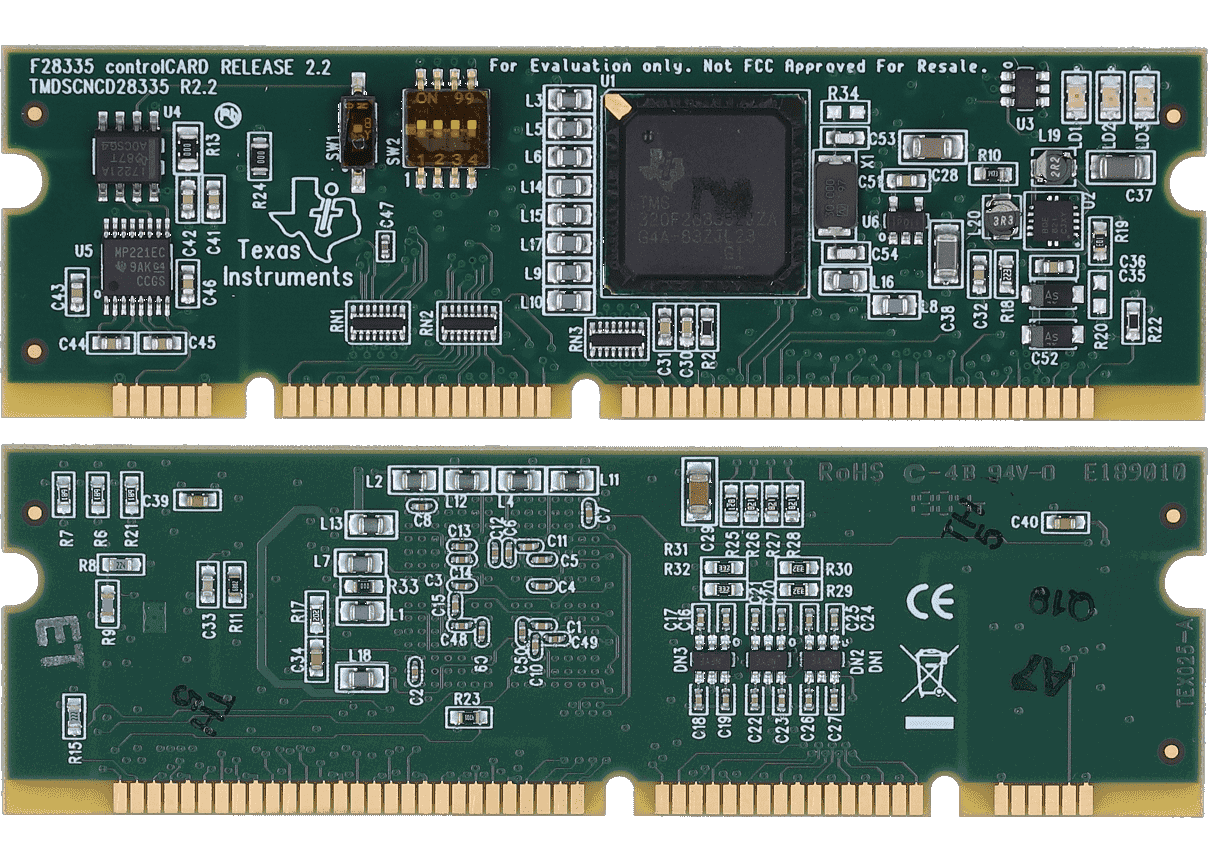
\includegraphics[scale=0.22]{Imagenes/ControlCARD.png}
    \caption{Controlador digital de señales modelo TMS320F28335 de la linea C2000, en su paquete de evaluación tipo ControlCARD, para inserción en slot DIMM-100.}
    \label{ControlCARD}
\end{figure}

El DSC fue seleccionado principalmente por su disponibilidad en el laboratorio, además de que ya fue utilizado en otros proyectos que pueden ser usados como referencia a la hora de diseñar el módulo. En cualquier caso, este controlador resulta apropiado para ser integrado a nuestro sistema, por su capacidad de procesamiento en tiempo real, su enorme cantidad y variedad de periféricos que permiten implementar diversas funcionalidades útiles, además de poseer una documentación muy completa por parte del fabricante.\\

\paragraph{Periféricos Importantes}